% !TeX spellcheck = hu_HU
% !TeX encoding = UTF-8
% !TeX program = xelatex
\documentclass[11pt,a4paper,oneside]{report}             % Single-side
%\documentclass[11pt,a4paper,twoside,openright]{report}  % Duplex

\input{include/packages}

\newcommand{\vikszerzoVezeteknev}{Szilágyi}
\newcommand{\vikszerzoKeresztnev}{Gábor}

\newcommand{\vikkonzulensAMegszolitas}{}
\newcommand{\vikkonzulensAVezeteknev}{Vörös}
\newcommand{\vikkonzulensAKeresztnev}{András}

\newcommand{\vikkonzulensBMegszolitas}{}
\newcommand{\vikkonzulensBVezeteknev}{Búr}
\newcommand{\vikkonzulensBKeresztnev}{Márton}

\newcommand{\vikkonzulensCMegszolitas}{}
\newcommand{\vikkonzulensCVezeteknev}{}
\newcommand{\vikkonzulensCKeresztnev}{}

\newcommand{\vikcim}{Monitoring of cyber-physical systems based on graph pattern matching} % Cím
\newcommand{\viktanszek}{\bmemit} % Tanszék
\newcommand{\vikdoktipus}{\msc} % Dokumentum típusa (\bsc vagy \msc)
\newcommand{\vikmunkatipusat}{diplomaterver} % a "hallgató nyilatkozat" részhez: szakdolgozatot vagy diplomatervet

\input{include/tdk-variables}
\newcommand{\szerzoMeta}{\vikszerzoVezeteknev{} \vikszerzoKeresztnev} % egy szerző esetén
%\newcommand{\szerzoMeta}{\vikszerzoVezeteknev{} \vikszerzoKeresztnev, \tdkszerzoB} % két szerző esetén

% Beállítások magyar nyelvű dolgozathoz
%\input{include/thesis-hu}
% Settings for English documents
\input{include/thesis-en}

\input{include/preamble}

%--------------------------------------------------------------------------------------
% Table of contents and the main text
%--------------------------------------------------------------------------------------
\begin{document}


\selectthesislanguage


%~~~~~~~~~~~~~~~~~~~~~~~~~~~~~~~~~~~~~~~~~~~~~~~~~~~~~~~~~~~~~~~~~~~~~~~~~~~~~~~~~~~~~~
\include{include/titlepage}		   % Szakdolgozat/Diplomaterv címlap
%\include{include/titlepage-tdk}	% TDK címlap
%\include{include/titlepage-otdk}   % OTDK címlap


% Table of Contents
%~~~~~~~~~~~~~~~~~~~~~~~~~~~~~~~~~~~~~~~~~~~~~~~~~~~~~~~~~~~~~~~~~~~~~~~~~~~~~~~~~~~~~~
\tableofcontents\vfill


% Declaration and Abstract
%~~~~~~~~~~~~~~~~~~~~~~~~~~~~~~~~~~~~~~~~~~~~~~~~~~~~~~~~~~~~~~~~~~~~~~~~~~~~~~~~~~~~~~
\include{include/declaration} 
\pagenumbering{roman}
\setcounter{page}{1}

\selecthungarian

%----------------------------------------------------------------------------
% Abstract in Hungarian
%----------------------------------------------------------------------------
\chapter*{Kivonat}\addcontentsline{toc}{chapter}{Kivonat}

A technológia fejlődésével rohamosan jelennek meg a kiberfizikai rendszerek egyre több tradicionális területen is: a vasúti rendszerek, robot rendszerek megfigyelését egyre több szenzor végzi, autók egymással kommunikálnak, és gyakran már önvezető funkcióval is rendelkeznek. Jellemzője ezen rendszereknek, hogy nagy mennyiségű szenzor adatot kell feldolgozniuk, és a rendelkezésre álló információk alapján gyorsan kell reagálniuk a környezet változásaira.

A kiberfizikai rendszerek gyakran kritikus feladatokat látnak el, ahol elengedhetetlen a helyes működés. Ennek biztosítására azonban nem mindig elegendőek a tradicionális, biztonságkritikus rendszerek esetén alkalmazott megközelítések, hiszen a gyorsan változó környezet, az alkalmazott intelligens megoldások és az elosztottság nem teszi lehetővé a tervezési idejű ellenőrzést. Erre nyújthat megoldást a futás idejű ellenőrzés, amelyre többféle megközelítés is létezik. Az időbeli viselkedéseket jellemzően automata formalizmusok segítségével és temporális nyelvekkel, míg a strukturális felépítést és adat jellegű viselkedést gráfminták segítségével tudjuk specifikálni és gráfmintaillesztés segítségével ellenőrizni. Az irodalomban is több megközelítés ismert, mi ezeket továbbfejlesztve egy olyan gráfmintaillesztés alapú elosztott ellenőrzést megvalósító keretrendszert terveztünk, amely képes egyrészt az elosztott rendszer lokális tulajdonságait vizsgálni, továbbá ezek alapján a rendszer állapotára következtetni és a lehetséges hibákat jelezni.

A keretrendszer egy nyílt forráskódú gráfmintaillesztő rendszerre épül. Munkánk során ezt egészítettük ki új algoritmusokkal, hogy a gráfminta specifikációk bővebb körét tudjuk támogatni. Amennyiben az ellenőrzéshez szükséges, az elosztottan futtatott ellenőrzések eredményeiből automatikusan számítjuk a rendszer új állapotát. Nyelvi támogatást adunk a szenzor adatok feldolgozására és a tudásbázisba való integrálásának támogatására. Az általunk fejlesztett gráfmintaillesztés alapú keretrendszerrel támogatjuk az elosztott kiberfizikai rendszerek ellenőrzését, és a megközelítésünk működését egy esettanulmány segítségével demonstráljuk.



\vfill
\selectenglish


%----------------------------------------------------------------------------
% Abstract in English
%----------------------------------------------------------------------------
\chapter*{Abstract}\addcontentsline{toc}{chapter}{Abstract}

The rapid development of technology leads to the rise of cyber-physical systems even in the field of safety critical systems like railway, robot, and self-driving car systems. Cyber-physical systems process a huge amount of data coming from sensors and other information sources and it often has to provide real-time feedback and reaction.

Cyber-physical systems are often critical, which means that their failure can lead to serious injuries or even loss of human lives. Ensuring correctness is an important issue, however traditional design-time verification approaches can not be applied due to the complex interaction with the environment, the distributed behavior and the intelligent controller solutions. Runtime analysis provides a solution where graph-based specification languages and analysis algorithms are the proper means to analyze the behavior of cyber-physical systems at runtime. Existing approaches from the literature formed the basis of our work: we developed a distributed runtime verification framework to analyze the local behavior of the components and ensure the global correctness of the systems.

We developed a framework on top of an existing open-source solution. We extended the framework to support a richer set of possible specifications and we implemented the corresponding algorithms. We provided a language to support the integration of sensor information to the knowledge base and we also developed a simple language to decompose the graph specifications and distribute the analysis algorithm to the components. In case of complex global specifications, the algorithm collects the information from the various analysis components and infers the state of the system. The introduced framework was evaluated in a research project of the department and proved its usefulness.



\vfill
\selectthesislanguage

\newcounter{romanPage}
\setcounter{romanPage}{\value{page}}
\stepcounter{romanPage}    


% The main part of the thesis
%~~~~~~~~~~~~~~~~~~~~~~~~~~~~~~~~~~~~~~~~~~~~~~~~~~~~~~~~~~~~~~~~~~~~~~~~~~~~~~~~~~~~~~
\pagenumbering{arabic}

%----------------------------------------------------------------------------
\chapter{\bevezetes}
%----------------------------------------------------------------------------

Cyber-physial systems are used in various contexts. Factories, logistics and energy systems can utilize computers to improve quality, provide monitoring features, and ensure safety for them. In this thesis a framework is presented capable of generating monitoring code, thus helping the developement of cyber-physical systems. 

We use model-driven developement paradigm, meaning that models are the primary artifacts in the developement process for the framework. Monitoring components are not programmed manually, but generated by our framework based on the models defined by the developers of the system, who use the framework. 

In Chapter 2, a motivating example is presented to show the used approach on a concrete example. In Chapter 3, preliminaries are expound to clarify the used terms and concepts. Chapter 4 is an overview for the approach that the framework uses. In Chapter 5 the design time details are provided to show, how the system provides artifacts for monitoring. Chapter 6 shows how those generated artifacts work at runtime. In Chapter 7 we measure and evaluate the framework.
\chapter{Motivating example}

\todo{Újracsinálni ezt az egészet, ez így egy okádék}

The target of this work is the runtime verification of distributed CPS systems. As a motivating example, the MoDeS3~\cite{modes3} demonstrator platform is used. 

 MoDeS3 stands for Model-based Demonstrator for Smart and Safe Systems. Its main goal is to demonstrate the many cool and innovative ways in which open source modeling tools can be used for systems development in the age of Internet-of-Things.
 
 The case study is a railway system: users can control trains arbitrarily as long as it is not dangerous. Accidents and dangerous situations are detected using sensors embedded into the track: they sense the trespass of the trains and send this information to the controllers. It is important to note that this is just local information, so we have to ensure that it will be shared between the components. The system employs six BeagleBone Black (BBB) embedded computers to run the safety logic, configured as a distributed system, where each BBB is responsible for some track sections.

\begin{figure}[H]
	\begin{center}
		\includegraphics[width=\textwidth]{figures/modes.png}
	\end{center}
\end{figure}

\pagebreak
We use information from sensors perceiving the system's physical state to deduce if the state of the system is incorrect and/or dangerous. This is done by creating a structural model for the system and updating it based on sensor data coming from sensors. This model is graph based and we use graph pattern matching to find model parts indicating errors in the physical system.

Monitoring goals for this system are defined as graph patterns. The usage and efficiency of the developed framework are demonstrated by defining these goals, compiling them to monitoring codes and running them on variously distributed models. 



% célok és feladatok, amiket demonstrálni szeretnénk, monitoring goalok kiértékelése.S

%----------------------------------------------------------------------------
\chapter{Preliminaries}
%----------------------------------------------------------------------------

In this chapter, we revisit the background knowledge on graph-based modeling, and graph pattern matching. We also introduce the used terminology as it is crucial in the following chapters. At the end of the chapter, we show how the concepts of graph pattern matching can be extended to run over distributed systems.

\section{Graph-based modeling}

Structural and behavioral modeling of systems is often done using graphs. 
Graphs are useful as they are easy to understand, intuitive to use, and lots of existing algorithms can be used to process them. 
As our model-based approach introduced in the framework relies on graphs as a representation, in this section, graph-based modeling is presented.

A directed graph consists of a set of nodes and a set of edges, where edges are ordered pairs of two nodes. An edge has a \emph{source} node and a \emph{target} node. 
Graphs can be extended to represent models by adding extra information, such as:
\begin{itemize}
	\item assigning a type to each node
	\item assigning a type to each edge that specifies the types of the source and the target node
	\item supplying nodes with attributes and attribute values (e.g.\ name)
\end{itemize}


\begin{figure}[H]
	\begin{center}
		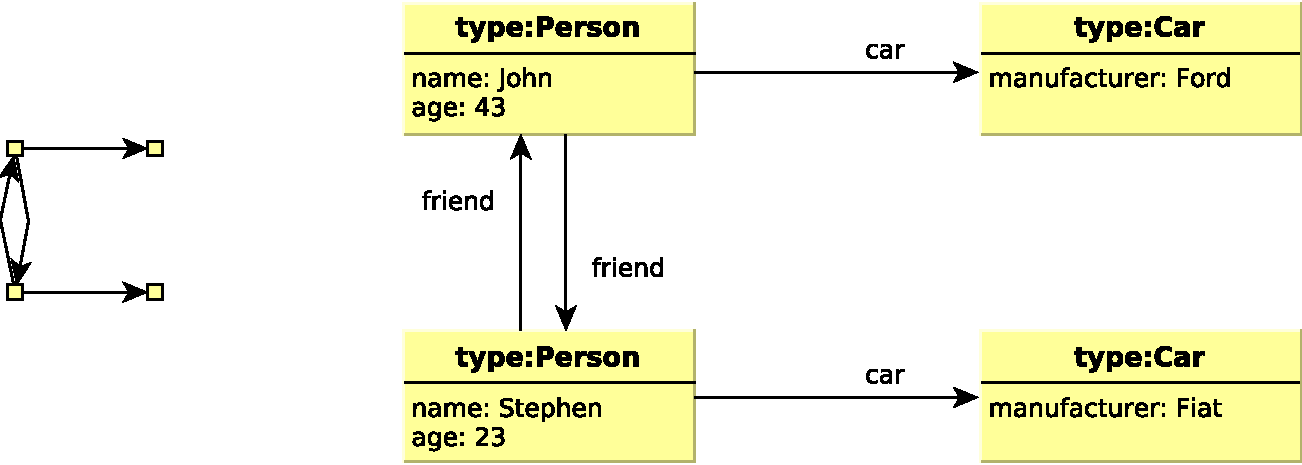
\includegraphics[width=\textwidth]{figures/graphs.pdf}
		\caption{Basic graph (left), and extended (right) }
		\label{fig:graphs}
	\end{center}
\end{figure}

To be consistent with the terminology used in software engineering, we also use the term \emph{object} for a typed node with attributes and \emph{reference} for a typed edge. 

A metamodel is a model, that defines how the graph model of a system is built up:
\begin{itemize}
	\item what type of objects exist
	\item what kind of attributes can a node of a certain type have
	\item what type of references exist and what type of object can be its source and target node
	\item multiplicity restriction for references and attributes
	\item hierarchical relationship between types
\end{itemize}

\autoref{fig:metamodel} shows some of these concepts. The upper part is a metamodel, and the lower is an instance model, that satisfies the rules defined by the metamodel: There can be 3 types of objects: \texttt{ModelElement}, \texttt{Train} and \texttt{RailRoadElement}. All instances of \texttt{ModelElement} has an \texttt{id}. Both of \texttt{Train} and \texttt{RailRodeElement} are a subtype of \texttt{ModelElement} which means, that each instance of the subtype works as an instance of the supertype as well.
\begin{figure}[h]
	\begin{center}
		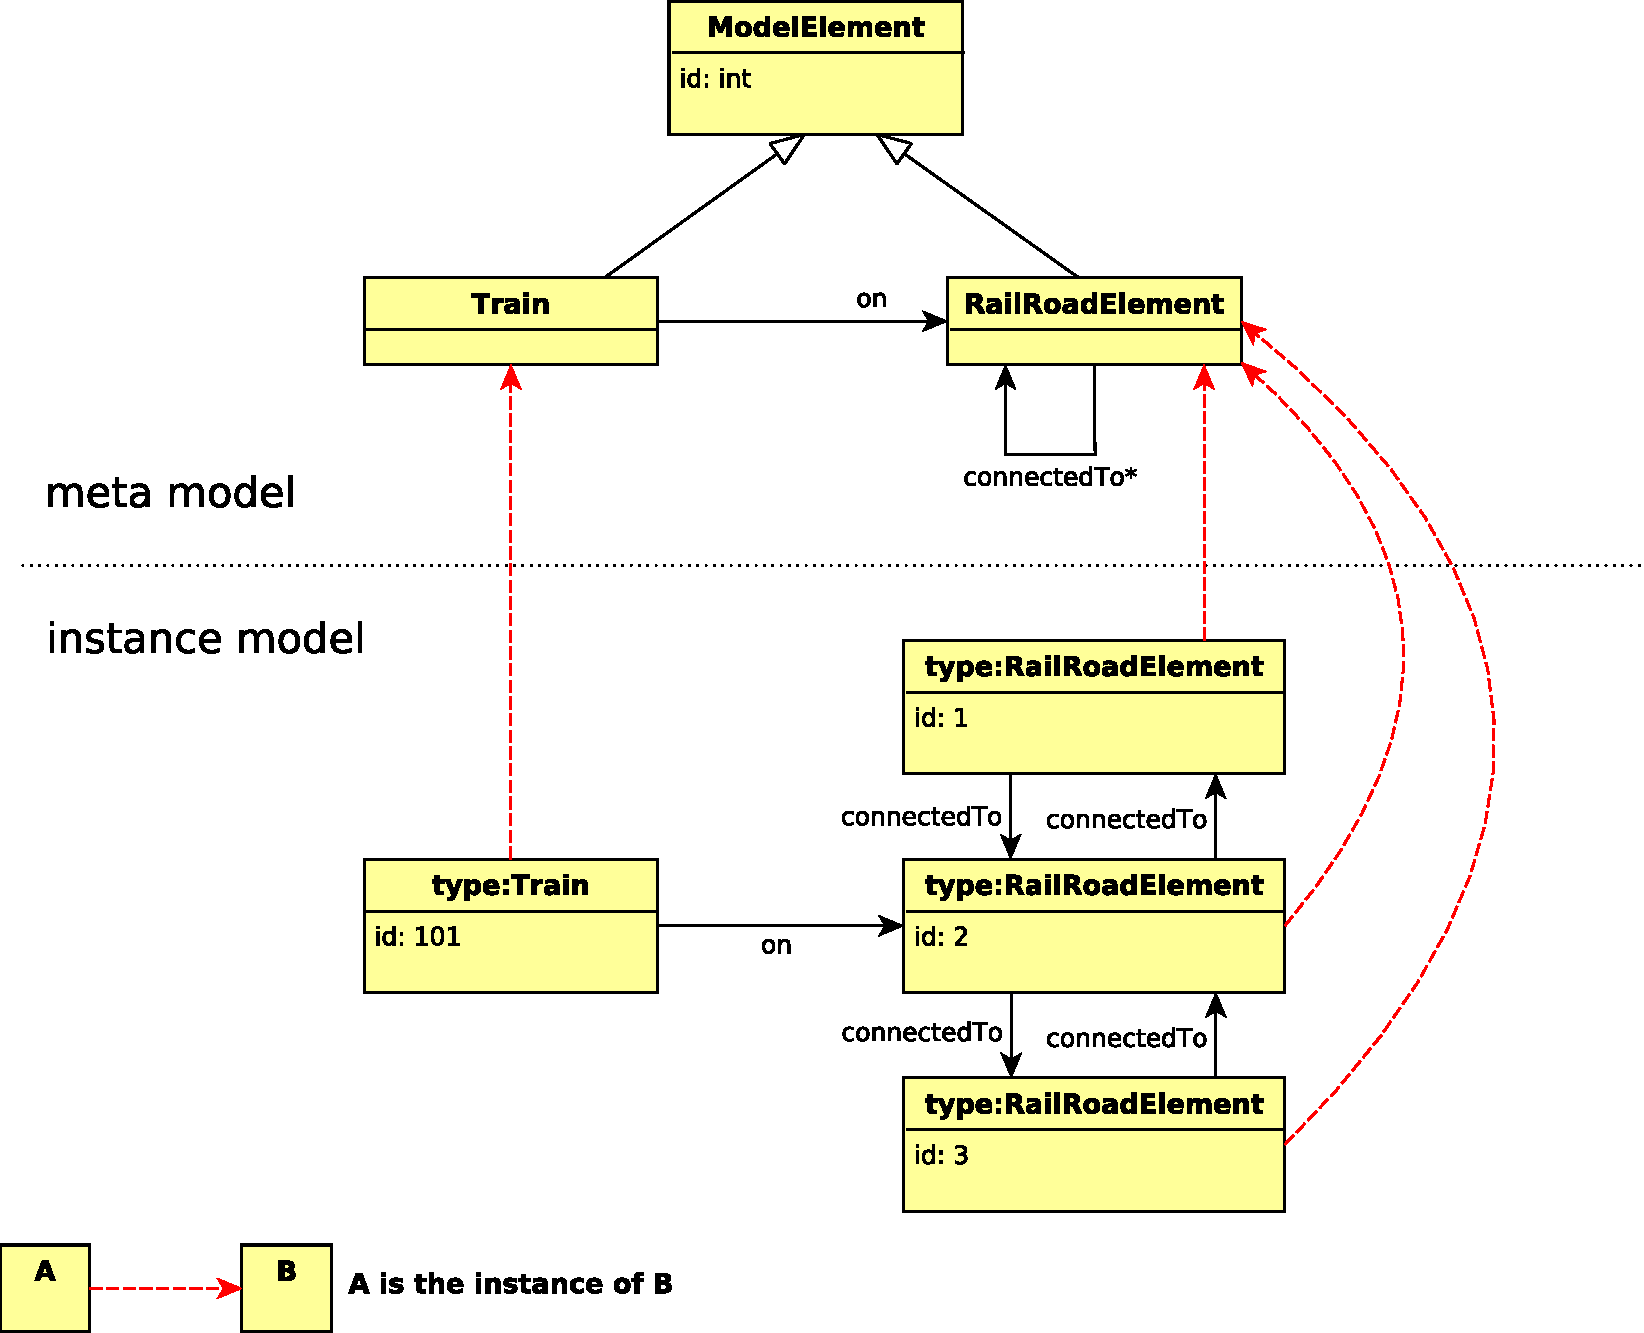
\includegraphics[width=\textwidth]{figures/metamodel.pdf}
		\caption{ Example of a metamodel and an instance model }
		\label{fig:metamodel}
	\end{center}
\end{figure}


\section{Domain and runtime modeling}

In this framework, we use graph-based models to represent the current state of the system. 
The state and the operating context of the system are captured in a model called the \emph{live model} or \emph{runtime model} \cite{Szvetits2013, DBLP:journals/computer/BlairBF09}.
It is updated with sensor data and information from other sources, so the model captures the physical system's latest known state.
This model is used for runtime verification.
While the model is being continuously updated it is also analyzed using graph pattern matching to find parts of the model that may imply error in the system.

An example of a live model is depicted in \autoref{fig:live-models}. As the train with \texttt{id}=105 is moving from the segment with \texttt{id}=1 to segment with \texttt{id}=2, the appropriate railway sensors send updates to the model, which is modified to represent, that the train is on an other segment.




\begin{figure}[H]
	\begin{center}
		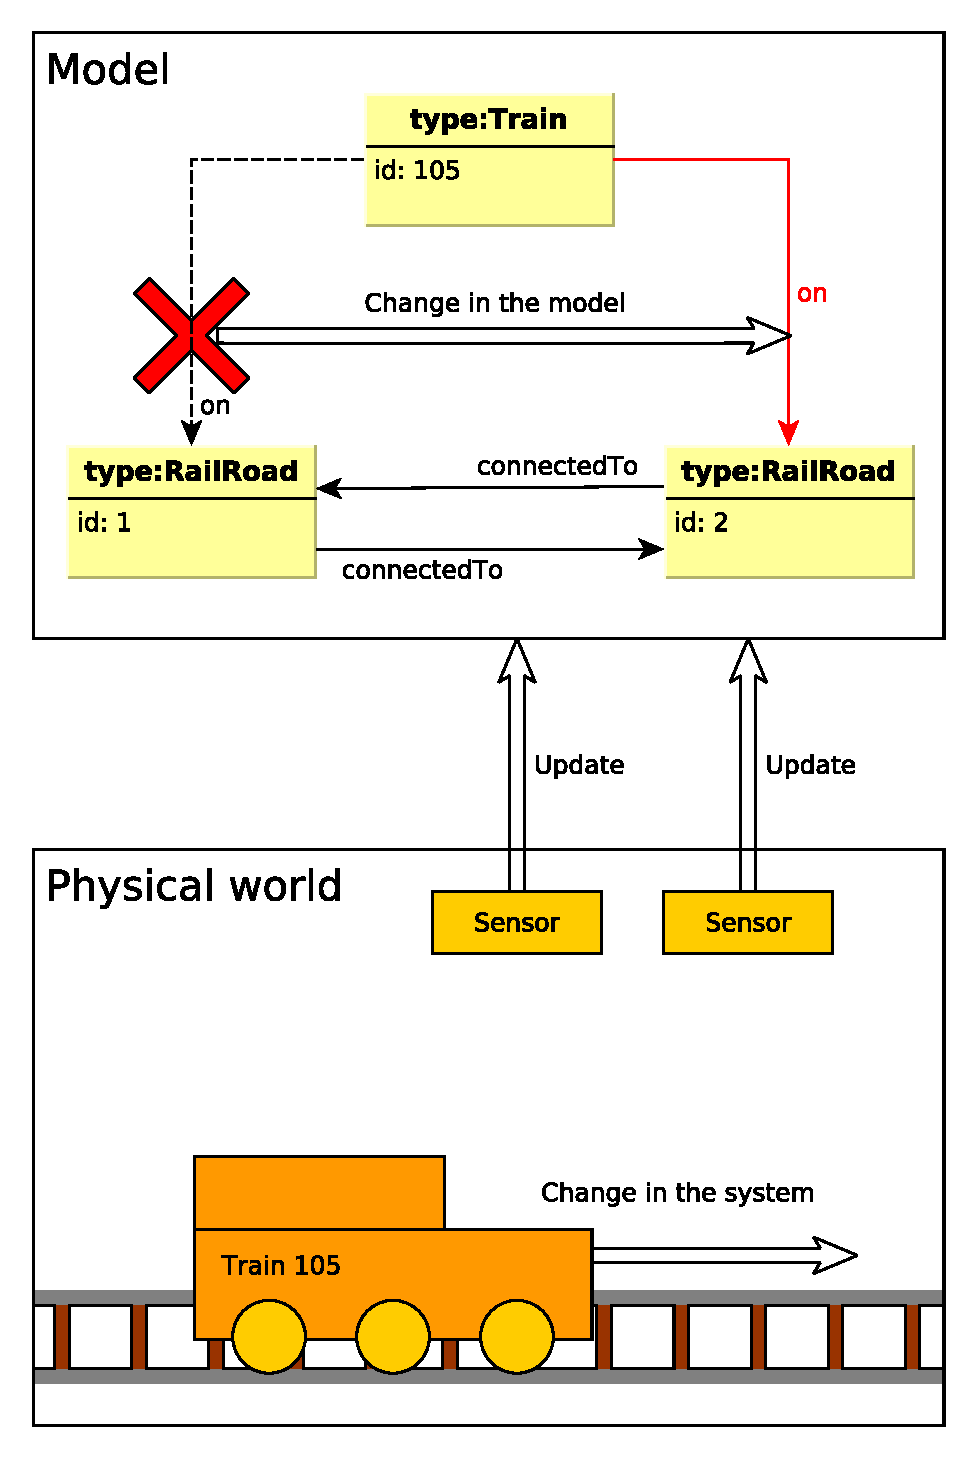
\includegraphics[width=0.7\textwidth]{figures/live-models.pdf}
		\caption{Live model updating}
		\label{fig:live-models}
	\end{center}
\end{figure}

\section{Foundations of graph pattern matching}
\label{section:gpmc}

\todo{Marci tanácsait bevezetni, ha frissebb leszek}
\todo{Tetszőleges kifejezéssel lehet gráf patternt adni, viszont a viatra és a local search miatt adott egy értelmes formához kötni magunkat}

The goal of graph pattern matching is to find all subgraphs of a graph meeting a certain criteria, defined by a \emph{graph pattern}.

We define the domain of an extended graph as the union of 
\begin{itemize}
	\item the set of the vertices of the graph
	\item and the set of data values (Strings, numbers, boolean values, and enumeration literals), that can be assigned to the attributes of its vertices
\end{itemize}

A \emph{graph pattern} is a predicate, and its  domain is the domain of the extended graph.
A \emph{pattern match} is a tuple of elements from the graph domain, that satisfies the predicate.
A pattern's \emph{match set} is the truth set of the predicate, i.e.\ the set of tuples that satisfies the predicate.
A \emph{graph query} is a program or execution plan capable of calculating the match set of a graph pattern on a given graph. 



We build up graph patterns with a modified\footnote{ Universal quantification and functions of terms are not included } first-order logical formula the following way:
\begin{itemize}
	\item Terms can be variables and constants, constants only refer to data values.
	\item A constraint is a predicate evaluated over terms. 
	\item A formula can be a constraint or an expression composed of logical connectives (and, or) and existential quantifier ($\exists{}$) used with another formula.
	\item The graph pattern itself is a formula.
\end{itemize}

We use the following constraints as basic elements of graph patterns:

\begin{itemize}
	\item Type -- Satisfied, when the variable's value is a vertex of a given type
	\newline Type(Variable)
	
	\item Reference -- Satisfied, when an edge with a given type exists from the first variable's value to the second variable's value (vertex only)
	\newline ReferenceName(Source variable, Target variable)
	
	\item Attribute -- Satisfied, when a variable value is a vertex, which's attribute is the same as another variable's value (data).
	\newline AttributeName(variable of vertex, variable of attribute value)
		
	\item Equality -- two variable's values are the same
	\newline $\mathit{var1} = \mathit{var2}$
		
	\item Inequality -- two variable's values are different
	\newline $\mathit{var1} \neq \mathit{var2}$
	
	\item Pattern match -- a tuple of variable values are a match of another pattern	
	\newline $\text{PatternName}(\mathit{v1}, \mathit{v2}, \dots{})$.
	
	\item Negative pattern match -- a tuple of variable values are not a match of another pattern	
	\newline $\text{neg PatternName}(\mathit{v1}, \mathit{v2}, \dots{})$.
	
	\item Pattern count -- Counts the matches of a pattern.
	\newline $v_{out} = \text{count PatternName}(\mathit{v1}, \mathit{v2}, \dots{})$.
\end{itemize}

We can also use a visual representation to illustrate a graph pattern, although a textual language (VQL) is used in the framework. 
\autoref{fig:pattern-visual} shows how different graph pattern representations work. The pattern on the figure means, that two element is a \texttt{RailRoadElement} with only one \texttt{RailRoadElement} between them, and they have trains on them.



\begin{figure}[H]
	\begin{center}
		
		\begin{minipage}[c]{\textwidth}
			\begin{minipage}[r]{\textwidth}
				\hfill
				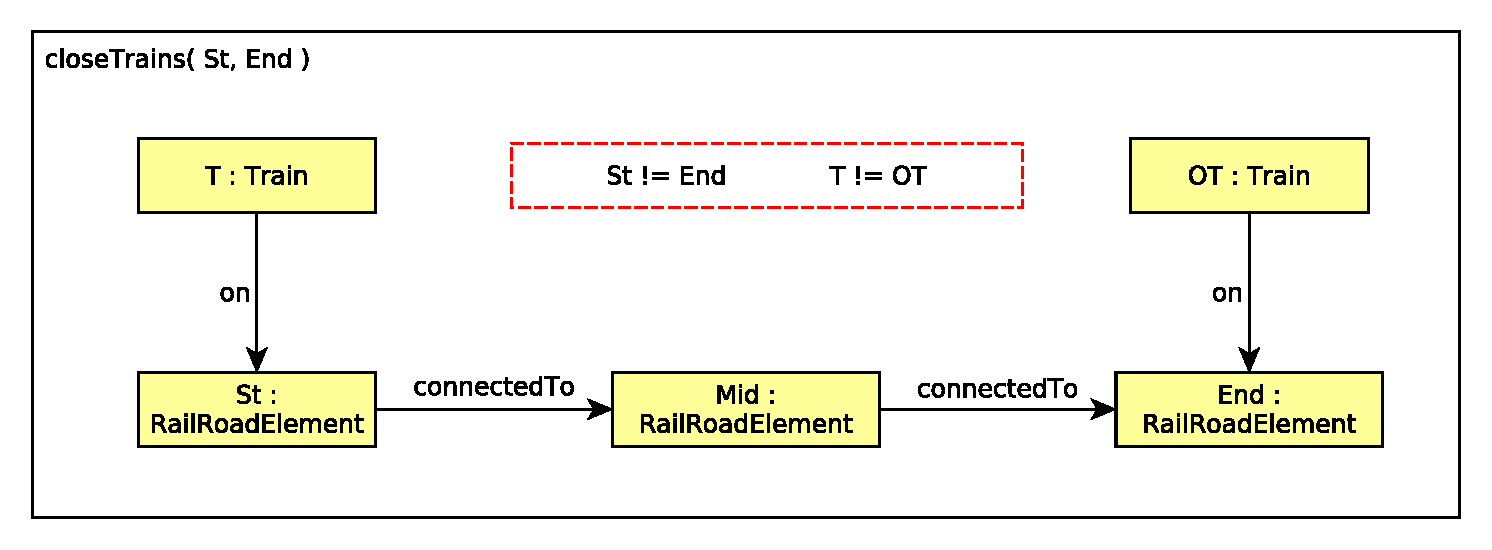
\includegraphics[width=\textwidth]{figures/closeTrains-pattern.pdf}
			\end{minipage}
			\hfill
			\begin{minipage}[c]{0.45\textwidth}
\begin{lstlisting}[language=vql]
pattern CloseTrains(St, End) {
	Train.on(T,St);
	Train.on(OT, End);
	RailRoadElement.connectedTo(St,Mid);
	RailRoadElement.connectedTo(Mid, end);
	T != OT;
	St != End;
}
\end{lstlisting}			
			\end{minipage}
			\hfill
			\begin{minipage}[l]{0.45\textwidth}
				
\begin{equation*}
\begin{array}{@{}l@{}}

\text{CloseTrains}(St, End) = \\
\exists{T} \  \exists{OT}\; \exists{Mid} ( \\
\text{on}(T, St)  \  \wedge \\
\text{on}(OT, End)  \  \wedge \\
\text{connectedTo}(St, Mid)  \  \wedge \\
\text{connectedTo}(Mid, End)  \  \wedge \\
\text{T} \neq OT  \  \wedge \\
\text{St} \neq End )
\end{array}
\end{equation*}
			
			\end{minipage}
		\end{minipage}
		\caption{CloseTrains pattern visualised (top), as defined in VQL (bottom left) and as a first-order logic expression (bottom right)}
		\label{fig:pattern-visual}
	\end{center}
\end{figure}



\section{Local search-based graph pattern matching}

Local search refers to a family of algorithms solving problems involving a search space. 
Local search starts from a candidate solution for a problem, then searches by applying local changes: moving to better neighboring solutions until eligible solutions are found.

Local search can also be used to find a match set for a graph pattern in a graph.
It is also a memory-efficient alternative for RETE algorithm in \viatra{}~\cite{bur-marton-msc}.
In our system, we use local search-based graph pattern matching. 

We define \emph{pattern body} as a subexpression of the graph pattern which has the following structure:
\begin{equation*}
\begin{array}{@{}c@{}}
\exists{\bar{x}} 
(\text{Constr}_{11}(\bar{p},\bar{x} ) \, \wedge \, 
 \text{Constr}_{12}(\bar{p},\bar{x} ) \, \wedge \, \dots{})
\end{array}
\end{equation*}
where $\bar{p}$ is the list of parameters, $\bar{v}$ is the list of variables that occur in the constraints.

In the following, we only use graph patterns composed by pattern bodies using the \emph{or} logical connective

\begin{equation*}
\begin{array}{@{}r@{}l@{}l@{}l@{}l@{}}
Pattern(p1, p2, \dots) = \;
& \exists{\bar{x}} ( & 
(\text{Constr}_{11}(\bar{p},\bar{x} ) & \, \wedge \, \text{Constr}_{12}(\bar{p},\bar{x} ) & \, \wedge \, \dots{}) \: \vee \\

& \exists{\bar{y}} & 
(\text{Constr}_{21}(\bar{p},\bar{y} ) & \, \wedge \, \text{Constr}_{22}(\bar{p},\bar{y} ) & \, \wedge \, \dots{}) \: \vee \\
& \dots{}
\end{array}
\end{equation*}

As VQL permits only this structure, the user must give the patterns in this form. This can be achieved by different transformations of the pattern, such as extracting negated expressions to subpatterns  and use negative pattern match constraint instead.

We can find the match set of this expression, by finding the match sets of all the pattern bodies as distinct predicates on the parameters, and taking their union.
The problem now is the following: find all variable bindings, which satisfies the constraints of the body.

\emph{Matching frame} of a body is defined as a partial function from variables to the domain of the graph i.e.\ as a partial variable binding.
A variable is bound in the frame, if it is mapped to a value, otherwise it is unbound.

Then the algorithm is the following:
\begin{enumerate}
	
\item
Let $C = (C_1, C_2, \dots{}, C_n )$ be the list of constraints in a given order.

\item 
Construct the frame, where all of the variables are unbound.

\item 
Starting from the first constraint:
	\begin{enumerate}
		\item 
		If all of the variables occurring in the constraint are bound in the current frame, then check if these values satisfies the constraint. 
		\begin{itemize}
			\item If they satisfy, then continue with the next constraint. If there are no more constraint, project this frame to the parameters and add it to the \mbox{match set}.
			\item if not, backtrack.
		\end{itemize}
		
		\item 
		If some variable occurring in the constraint are unbound, find all the possible values, that satisfy the constraints.
		Construct a frame for each of them, and continue for each frame at the next constraint. If there are no more constraints, project this frame to the parameters and add it to the match set.	
	\end{enumerate}	
\end{enumerate}
	
	
\begin{figure}[h]
	\begin{center}
		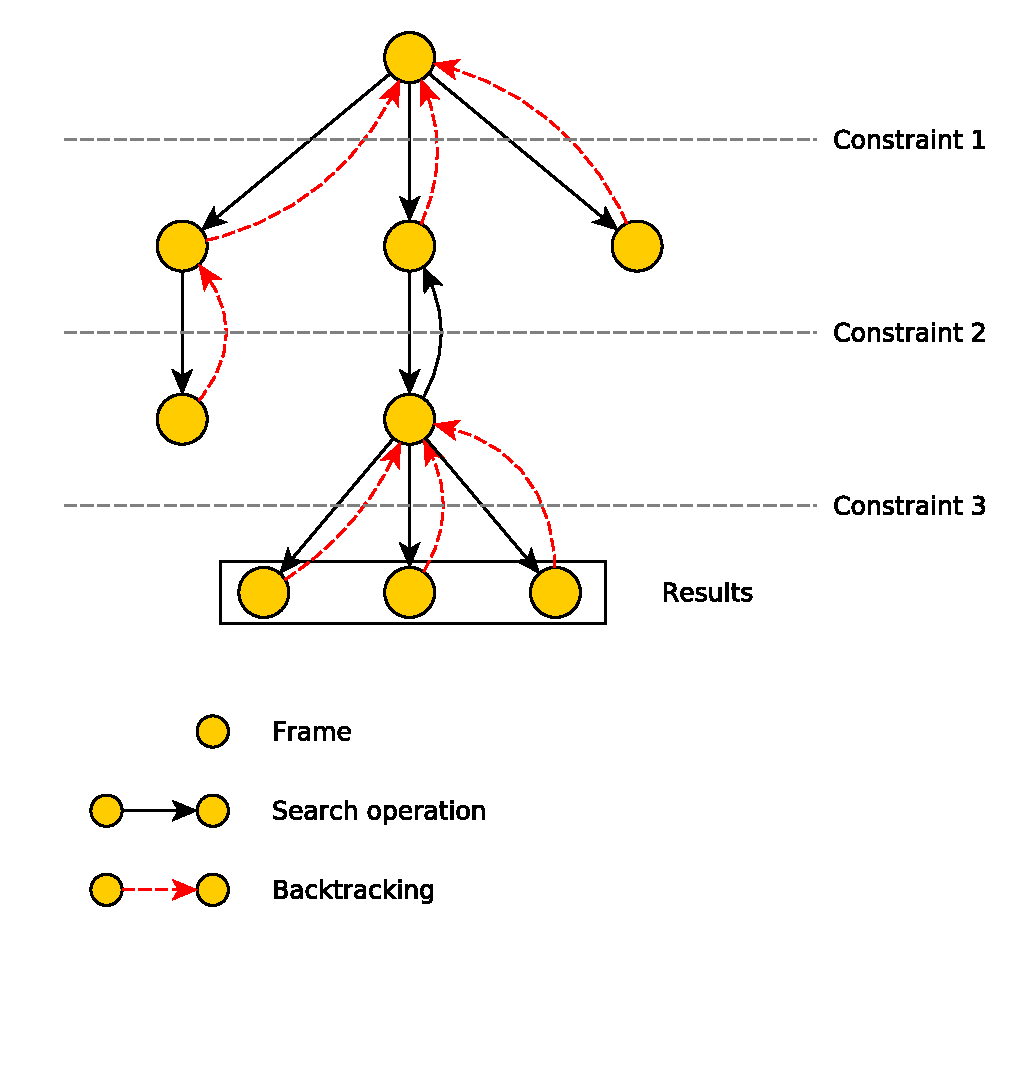
\includegraphics[width=0.7\textwidth]{figures/localsearch.pdf}
		\caption{Handling distributed models and cross-references}
		\label{fig:localsearch}
	\end{center}
\end{figure}
	
This algorithm is depicted in \autoref{fig:localsearch}. 
We can see, that it is a depth-first search in the space of frames. 
Because already bound variables are not modified, we can conclude the following:
\begin{itemize}
	\item 
	The search space is a tree, because all of the children of a frame will bind a variable differently, and these values are not changed in the subtree.
	\item
	At the $i$th layer of the tree, the first $i$ constraint is satisfied by the frame, as a child node does not modify already bound variables.
		
\end{itemize}

This means, that after computing the last constraint, the variable binding satisfies all the constraints, so it can be projected to the variables to form a solution.

We use depth-first search, because it uses less memory. Also generating depth-first search code is easy and efficient, as the layers are well defined. This way search can be easily implemented using nested for loops.

\subsection{Local search plan}
With a given order of the constraints, at the evaluation of the $i$th constraint we know what variables are already bound. Thus we know what kind of operation we will have to execute to generate the next frame which will satisfy the constraint.

A \emph{search operation} is an operation, that constructs the frames from the current frame, so they satisfy a given constraint.
\begin{itemize}
	\item 
	A \emph{check operation} is a search operation, which checks, whether the frame satisfies the given constraint. If it is, then the next frame is the same as the current frame, otherwise there are no next frames. (see the algorithm at 3.(a))
	\item
	An \emph{extend operation} is a search operation, which construct the next frames as all the frame, that binds the unbound variables which occurs in the constraint in a way, that the constraints is satisfied. (see the algorithm at 3.(b))

\end{itemize}


\emph{Local search plan} is a sequence of search operations.

\section{Distributed computational platform}

% adatok diszjunkt halmazokra bontva különböző csomópontra
% az algoritmusok is elosztottak, nem lesz összegyűjtve az infó, úgy van kiértékelve, hogy nincs aki mindent látna a rendszerből

In this thesis, the phrase \emph{computing unit} is used to denote a physical or virtual execution component of the CPS that is capable of storing a part of the graph model and updates it to represent the current state of the physical world, eg.\ an embedded system or a virtual machine.

In distributed CPSs various sensors serve as data sources and these sensors are connected to different computing units of the platform. However, in order to be able to monitor the distributed system as a whole, computing units need to exchange data.
Sending the sensor data to one computing unit and evaluate on that can cause different problems: 
sensor data can be too large to be sent over network, the central node can be a SPOF~(Single Point of Failure), etc. 

In the presented framework the live model is distributed into the different computing units and the graph pattern matching algorithm itself runs in a distributed way. 
This eliminates the problem of central computers, but introduces complexity, that we must handle.
One of the problems is distributed model handling, and the other is how to execute queries efficiently on a distributed platform.




\begin{figure}[h]
	\begin{center}
		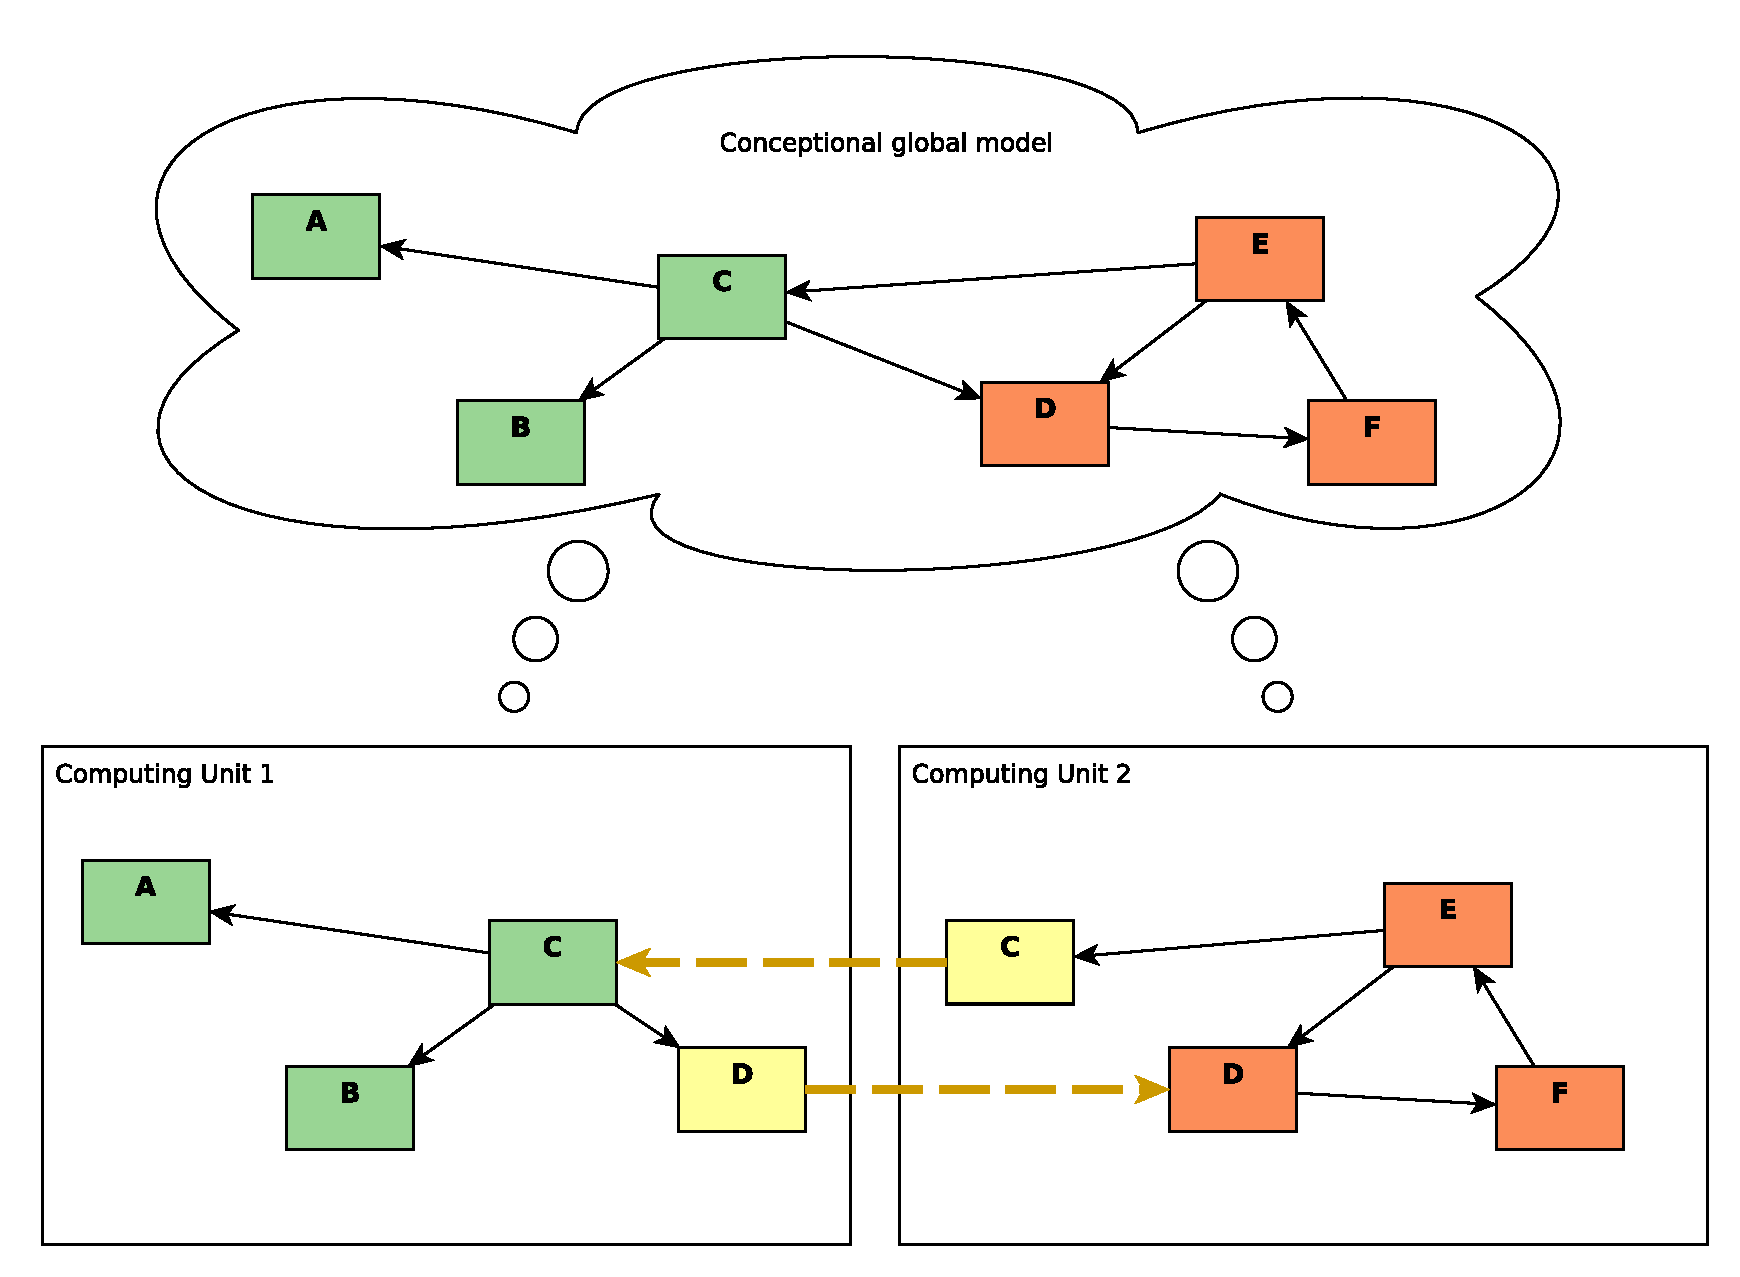
\includegraphics[width=\textwidth]{figures/distributed-model-handling.pdf}
		\caption{Handling distributed models and cross-references}
		\label{fig:distributed-model-handling}
	\end{center}
\end{figure}

\subsection{Distributed graph models}

In our framework each node in the graph is allocated to a computing unit. 
On that computing units, the node is called a \emph{local node}. 
In the context of other computing modules it is called a \emph{remote node}. 
Edges are stored in the computing module of their source node; 
If their target node is not a local node on that node, a \emph{proxy node} is used to substitute the remote node.
These concepts are illustrated in \autoref{fig:distributed-model-handling}.
From the perspective of Computing Unit 1, the green elements are local, and a red ones are remote. The yellow D is a proxy object which is used to represent the remote node in the reference from C to D.
A global model does not exist but computing units store partial models. Edges connecting elements of different computing units are stored by creating proxy elements on the computing unit of the source nodes. 


\subsection{Distributed query execution}

Distributed query execution is used in the framework to provide graph pattern matches
The purpose of distributed query execution is to run queries on distributed models on multiple computers. 
This introduces complexity, as we need to minimize network load, find matches that can span over multiple model parts, and provide low response times despite the distributed structure of the model.


\begin{figure}[h]
	\begin{center}
		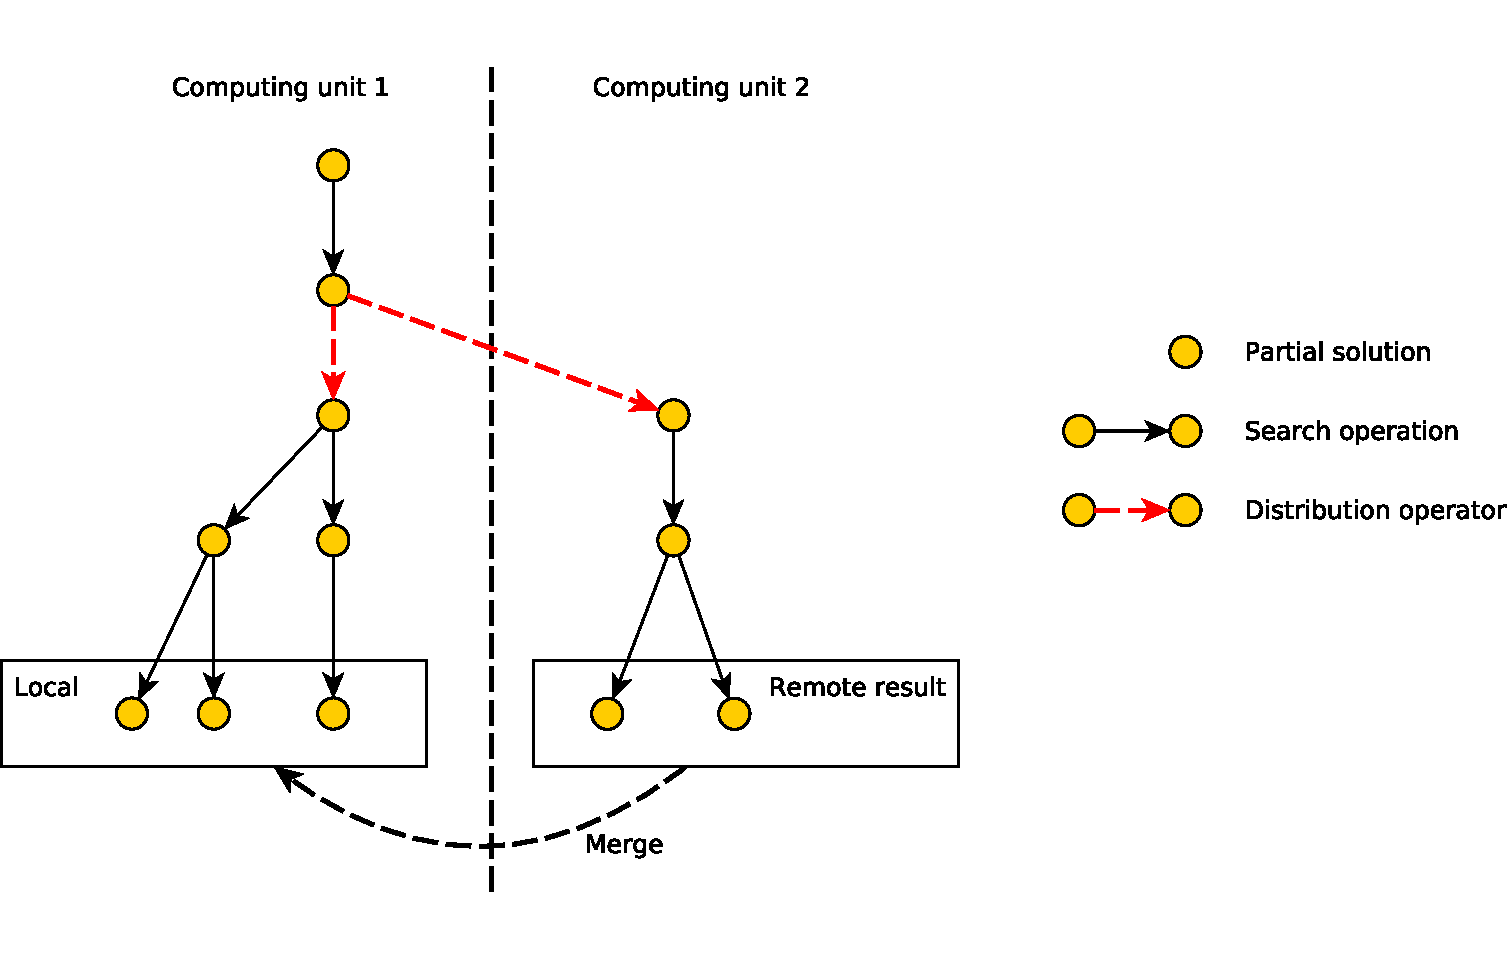
\includegraphics[width=\textwidth]{figures/distributed-ls.pdf}
		\caption{Distributed local search}
		\label{fig:distributed-ls}
	\end{center}
\end{figure}

In the framework, we extended local search-based graph pattern matching to work on distributed models.
This is achieved by doing the basic search operations locally, but create additional operations, which works in a distributed manner. 
Their mechanism is depicted on \autoref{fig:distributed-ls}.
These operations transmit the query execution to other computing units.
The other units continue to execute the query locally. When their results are calculated, they send it back to the caller.
The caller waits for the results and merges the local and remote results.

In this framework, we introduce two distributed operations:
\begin{itemize}
	\item Global distribution: globally distributes the query execution to all computing units (broadcast mechanics).
	\item Targeted distribution, distributes the query execution to the node, which contains a given model element.
\end{itemize}

The first can be used to globally iterate throw all elements of a given type. 
The latter is to help navigation through references, as references are stored locally.

A distributed local search plan can be calculated from a non-distributed one by the following:
\begin{itemize}
	\item If a search operation is based on reference constraint, we insert a targeted distribution operation before it to transmit the evaluation to the computing element containing the source variable.
	\item If a search operation is based on reference constraint, we insert global distribution operation before it to transmit the evaluation to all of the nodes, as any node can contain an object of that type.
\end{itemize}

This way, the distributed local search plan will have the same effect, but can be evaluated over distributed systems.


\section{Related work}

\newcommand{\mrt}{models\-@ run\-time\space}

%TODO mindenhol legyen meg, hogy latszodjon, mi az uj
%\paragraph{Runtime verification approaches.}
\subsubsection{Runtime verification approaches}
For continuously evolving and dynamic CPSs, an upfront design-time formal analysis needs to incorporate and check the robustness of component behavior in a wide range of contexts and families of configurations, %\cite{Lee2014}, 
which is a very complex challenge. Thus consistent system behavior is frequently ensured by runtime verification (RV) \cite{Leucker2009}, which checks (potentially incomplete) execution traces against formal specifications by synthesizing verified runtime monitors from provenly correct design models \cite{Mitsch2014,Joshi2017}.

\subsubsection{Runtime verification of distributed systems}
While there are several existing techniques for runtime verification of sequential programs available, the authors of \cite{Mostafa2015} claim that much less research was done in this area for distributed systems. Furthermore, they provide the first sound and complete algorithm for runtime monitoring of distributed systems based on the 3-valued semantics of LTL.

The recently introduced Brace framework~\cite{Zheng2016} supports RV in distributed resource-constrained environments by incorporating dedicated units in the system to support global evaluation of monitoring goals. There is also focus on evaluating LTL formulae in a fully distributed manner in \cite{Bauer2016} for components communicating on a synchronous bus in a real-time system.
Additionally, machine learning-based solution for scalable fault detection and diagnosis system is presented in \cite{Alippi2017} that builds on correlation between observable system properties.

\subsubsection{Distributed graph queries}
%TODO ezzel kapcsolatos eredmenyeket keresni
%TODO trinity
Highly efficient techniques for local-search based \cite{icgt2015} and incremental model queries \cite{scp2015} as part of the VIATRA framework were developed, which mainly builds on RETE networks as baseline technology. In \cite{models2014-iqd}, a distributed incremental graph query layer deployed over a cloud infrastructure with numerous optimizations was developed. 
Distributed graph query evaluation techniques were reported in \cite{Mitschke2014,Peters2014,Krause2014}, but none of these techniques considered an execution environment with resource-constrained computation units.

\subsubsection{Runtime models} 
The \mrt paradigm~\cite{DBLP:journals/computer/BlairBF09} serves as the conceptual basis for the Kevoree framework~\cite{Morin2014} (developed within the HEADS FP7 project). Other recent distributed, data-driven solutions include the Global Data Plane \cite{Zhang2015} and executable metamodels at runtime \cite{Vogel2014}. However, these frameworks currently offer very limited support for efficiently evaluating queries over a distributed runtime platform, which is the main focus of our current work.









%----------------------------------------------------------------------------
\chapter{Overview of the approach}
%----------------------------------------------------------------------------

%%
%% Futásidejű dolgok és kódgenerálás is!
%%

In this chapter I present the approach to monitoring of cyber-physical systems, that the developed framework uses. 


\begin{figure}[h]
	\begin{center}
		\includegraphics[width=\textwidth]{figures/fase-overview-crop.pdf}
	\end{center}
\end{figure}




%%
\chapter{Domain modeling and monitoring goal definition in EMF and \viatra{}}
%%

In this chapter the creation of initial artifacts is presented: domain models and graph patterns.
Domain modeling is an essential part of our framework, as the domain model defines the structure of the runtime live model, and affects the whole process. 
After the domain model is known, graph pattern can be specified, which will be used later in runtime analysis.
In the framework domain modeling are technologically backed up by EMF (Eclipse Modeling Framework), 
while graph pattern definition and processing are provided by \viatra{}.

\section{Eclipse Modeling Framework}


\begin{figure}
	\begin{center}
		\includegraphics[width=0.5\textwidth]{figures/EcoreHierarchy.png}
		\caption{Hierarchy of Ecore elements (Source: \cite{ecore-package}) }
		\label{fig:ecore-hierarchy}
	\end{center}
\end{figure}

\begin{figure}
	\begin{center}
		\includegraphics[width=\textwidth]{figures/EcoreRelations.png}
		\caption{Relations between Ecore elements (Source: \cite{ecore-package}) }
		\label{fig:ecore-relations}
	\end{center}
\end{figure}

Eclipse Modeling Framework (EMF) is an Eclipse based technology, which provides tools for model based developement: 
Ecore \cite{ecore-package} for metamodeling (Ecore actually defines a meta meta-model for metamodeling), and various tools like java code generation from ecore models, etc.

Ecore metamodeling is highly similar to defining class diagrams in UML, however, 
Ecore is more suitable for data and structural modeling: Interfaces are not a part of it, even though it can be substituted by abstract classes, as multiple inheritance is supported.

The hierarchy of Ecore elements can be seen on figure \ref{fig:ecore-hierarchy}, while its structure on \ref{fig:ecore-relations}
EObject is a base for everything, and its main purpuse to define the containment hierarchy of the model. 
EObjects can contain each other in a strict tree structure, circular containments are not permitted.
EModelElement expands EObject by giving the possibility to annotate them.

An Ecore model contains packages (EPackage). 
Packages have a namespace URI (nsURI), which can be used to refer it in other context eg.\ Viatra graph pattern definition.
Packages can contain other subpackages, classes (EClass), enumerations (EEnum), and data types (EDataType).

Classes have structural features: references and attributes (EStructuralFeature, EReference, EAttribute); also they have operations (EOperation).
References and attributes have multiplicity, defining their lower and upper bound is also possible.
ECore also provides tools to define containment hierarchy in the domain model itself: References can be containment or containing reference (considering direction of the reference). 
Two way navigation can be achieved by defining two reference and set them as the EOpposite of each other. A reference cannot be the EOpposite of itself, but its not a problem in most of the cases (eg.: \texttt{Human} class and \texttt{Spuse} reference). 

Multiple inheritance is supported for classes (eSuperTypes refers to direct base classes, and eAllSuperTypes for all transitively inherited base classes).

Besides classes, packages can contain enumerations and data types. 
Basic data types -- like EString, EInt, EBoolean etc.\ -- are defined by EMF, so its mostly never necessary to define others.
Enumerations are consists of EEnumLiterals. 
EEnumLiterals have an integral unique value, and its name is encapsulated in its EEnumerator instance.



	

\section{\viatra{} query language (VQL)}

As stated before, graph patterns can be defined using \viatra{} query language (VQL). 
The language syntax is simple, altough complex queries are not always self evident how to be expressed.

\subsection{Pattern definition}
Patterns and its bodies can be given by the \emph{pattern} keyword. 
Parameters must be specified after the parameter name in round brackets. 
Bodies of the pattern are given in curly brackets, separeted by the \emph{or} keyword

\begin{minipage}{\textwidth}
\begin{lstlisting}[language=vql]
pattern patternName( p1: Type1, p2: Type2){
... // Constraints for first body
} or {
... // Constraints for second body
} ...
\end{lstlisting}
\end{minipage}


\subsection{Constraints}
Constraints are given like statements. 
Each constraint is followed by a semicolon.

\vspace{\abovedisplayskip}
\begin{minipage}{\textwidth}
Type constraint can be given by specifying the type, then the object in round brackets.
\begin{lstlisting}[language=vql]
pattern patternName( o ){
	Type(o);
}
\end{lstlisting}
\end{minipage}
\vspace{\belowdisplayskip}

\begin{minipage}{\textwidth}
Reference constraint can be given by specifying which type's which reference must be checked, then giving the source and target variables in round brackets:
\begin{lstlisting}[language=vql]
pattern patternName( p1: Person, p2: Person ){
	Person.friend(p1, p2);
}
\end{lstlisting}
\end{minipage}
\vspace{\belowdisplayskip}

\begin{minipage}{\textwidth}
Other patterns can be used as constraint with the find keyword:
\begin{lstlisting}[language=vql]
pattern patternName( p1: Type1, p2: Type2, p3: Type3 ){
	find otherPatternName(p1, p2);
	find otherPatternName(p2, p3);
}
\end{lstlisting}

Also we can use underscore instead of specifying parameters. 
This way the constraint is satisfied, if the pattern matches with anything in the place of underscores (existential quantification).
\begin{lstlisting}[language=vql]
pattern patternName( p1: Type1 ){
find otherPatternName(p1, _);
}
\end{lstlisting}

This is the same as the following (if x is not used anywhere else):
\begin{lstlisting}[language=vql]
pattern patternName( p1: Type1 ){
find otherPatternName(p1, x);
}
\end{lstlisting}
\end{minipage}
\vspace{\belowdisplayskip}

\begin{minipage}{\textwidth}
Negative application condition can be expressed by neg find keyword:
\begin{lstlisting}[language=vql]
pattern patternName( p1: Type1, p2: Type2 ){
	neg find otherPattern(p1, p2);
	Type1.reference(p1, p2);
}
\end{lstlisting}

Also, we can use underscore if we don't want that the other pattern match occurs with \emph{any} value at the underscores. ( ie.\ neg find can be used to express negated existential quantification along with negated expressions )

\begin{lstlisting}[language=vql]
pattern patternName( p1: Type1 ){
	neg find otherPattern(p1, _);
}
\end{lstlisting}
\end{minipage}
\vspace{\belowdisplayskip}

\todo{Ez nem ugyanaz mint az előző esetben}

\begin{minipage}{\textwidth}
The keyword check can be used to create a constraint, that a given a java (XBase) expression is true. The expression only can refer to attribute  variables (Variables refering to data types instead of graph nodes).
\begin{lstlisting}[language=vql]
pattern adultPerson( p: Person ){
	Person.age(p, age);
	check(age >= 18);
}
\end{lstlisting}
\end{minipage}
\vspace{\belowdisplayskip}

\begin{minipage}{\textwidth}
The keyword eval can be used to evaluate a java (XBase) expression on attribute variables and assign the result to another variable.
\begin{lstlisting}[language=vql]
pattern patternName( p1: Person, p2: Person, agesum : EInt ){
	Person.age(P1, a1);
	Person.age(P2, a2);
	agesum = eval(a1 + a2);
}
\end{lstlisting}
\end{minipage}
\vspace{\belowdisplayskip}



\todo{ count find, equality, inequality}

\subsection{Annotations}


\section{VQL examples from the case study}

\todo{TODO megcsinalni}


%%
\chapter{Generating query based monitoring components}
%%

After the domain model of the system is designed, and the graph queries are written, the monitoring components can be generated and deployed along with \cpp{} tools for modeling the domain.
As stated before, domain modeling and graph query definition are done using EMF and \viatra{} technologies.
In this chapter, I present how the monitoring components are generated from these artifacts.

From the metamodel, the framework generates the classes, which enables the programmer to model the system's state in \cpp{}.
Also, we generate the monitoring code for the system, which is basically the \cpp{} implementation of the planned graph queries. 
These graph queries are evaluated on the maintained \cpp{} model at runtime, to show if there are some problems in the system.

%%%%
%%%%
%%%%
		\section{Generating classes from the metamodel}
%%%%
%%%%
%%%%

The domain model consists of packages (EPackage), enumerations (EEnum) and classes (EClass).
From an EPackage, we generate a folder; Every source file originated from an elements from the package will be generated in that folder. 
We generate sources from each class and enumeration of the package, also we generate other artifacts for the package, like helper classes, or model handling tools.


\subsection{Mapping an EClass to \protect\cpp }


\todo{ábra szépítés}
\begin{figure}
	\begin{center}
		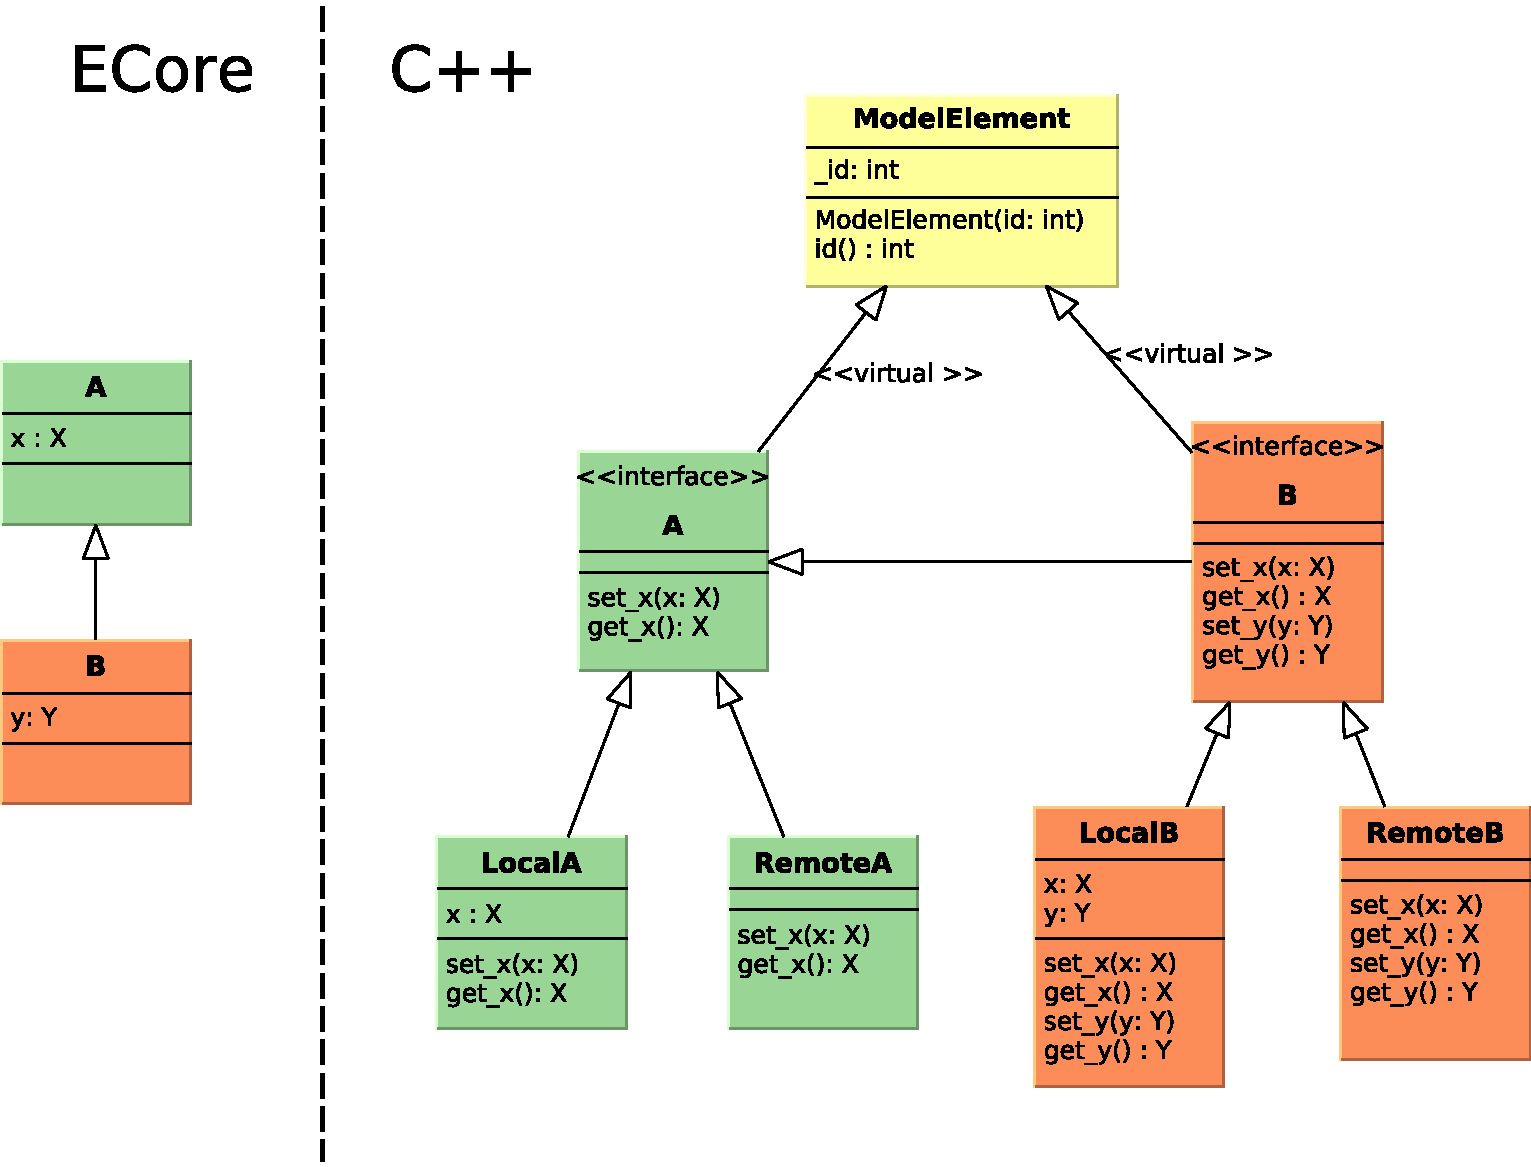
\includegraphics[width=\textwidth]{figures/eclass-to-cpp.pdf}
		\caption{Mapping of two EClasses, one inherited from the other (Left: EClasses, right: \protect\cpp{} classes) }
		\label{fig:eclass-to-cpp}
	\end{center}
\end{figure}


The EClasses of the metamodel are mapped to various \cpp{} classes, as depicted on \mbox{Figure~\ref{fig:eclass-to-cpp}}.
From each EClass we generate three \cpp{} classes:

\begin{itemize}
	\item An interface (abstract class with only pure virtual methods in \cpp{})
	\item A local class
	\item A remote class
\end{itemize}


The interface provides access to an instance of the EClass.
The local class implements the interface. It stores the attributes and references of the instances allocated to the local computing unit, and made them accessible by the methods of the implemented interface.
The remote class implements the interface, but are only used to substitute remote objects in references to them; 
Accessing its variables are not possible, because they are stored in another node. 

\subsection{Mapping an EEnum to \protect\cpp }

Enumerations are simply mapped to \cpp{} enum classes as depicted on Fig.\ref{fig:eenum-to-cpp}.

\begin{figure}[H]
	\begin{center}
		
		\begin{minipage}[c]{\textwidth}
		\begin{minipage}[r]{0.52\textwidth}
			\hfill
			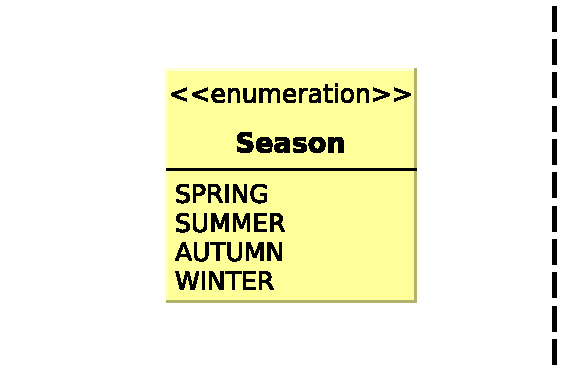
\includegraphics[width=0.735\textwidth]{figures/eenum-to-cpp.pdf}
		\end{minipage}
			\hspace{0.05\textwidth}
		\begin{minipage}[c]{0.25\textwidth}
\begin{lstlisting}[language=C++]
namespace Package{

enum class Season{
	SPRING = 0,
	SUMMER = 1,
	AUTUMN = 2,
	WINTER = 3
};

}
\end{lstlisting}			
		\end{minipage}
		\end{minipage}
		\caption{Mapping of an enumeration to \protect\cpp{} enum class }
		\label{fig:eenum-to-cpp}
	\end{center}
\end{figure}

\subsection{ Generating ModelRoot class }

A class called ModelRoot is also generated.
The purpose of ModelRoot is to handle the whole model of the system: 
It contains the instances of the classes and it keeps track of the objects by identifier.
It also provides a method to read in initial models from a json file.
The ModelRoot class is also the connection point between the monitoring components and the model.

\subsection{ Other sources }

For each package the framework generates
\begin{itemize}
	\item a header file containing forward declarations for each generated classes
	\item a header file including all the full declaration of classes
	\item a header file containing string conversion methods for enumerations, as \cpp{} lacks this feature in enum classes.
\end{itemize} 



%%%%
%%%%
%%%%
		\section{Overview of the query compilation workflow}
%%%%
%%%%
%%%%



The compilation of the queries of the CPS is depicted in fig. \ref{figure:query-compile-workflow}. 
First, vql files are parsed using EMF so their contents are loaded into a Pattern Model.
The Pattern Model are processed by \viatra{} and converted into PSystem representation of queries.
After that, we extend this representation with type information, as type information is more important in the \cpp{} generated code, than in the \viatra implementation of local search.
Then, we create the plan for query execution; We use the local search planner of \viatra{} fine tuned with our search operation cost function to improve performance of distributed queries. 
We also use some optimizations later to improve distributed performance. 
After the fully optimized plan is ready, we can construct the generator model describing the source code structure and generate the \cpp{} files.


\begin{figure}[h]
	\begin{center}
		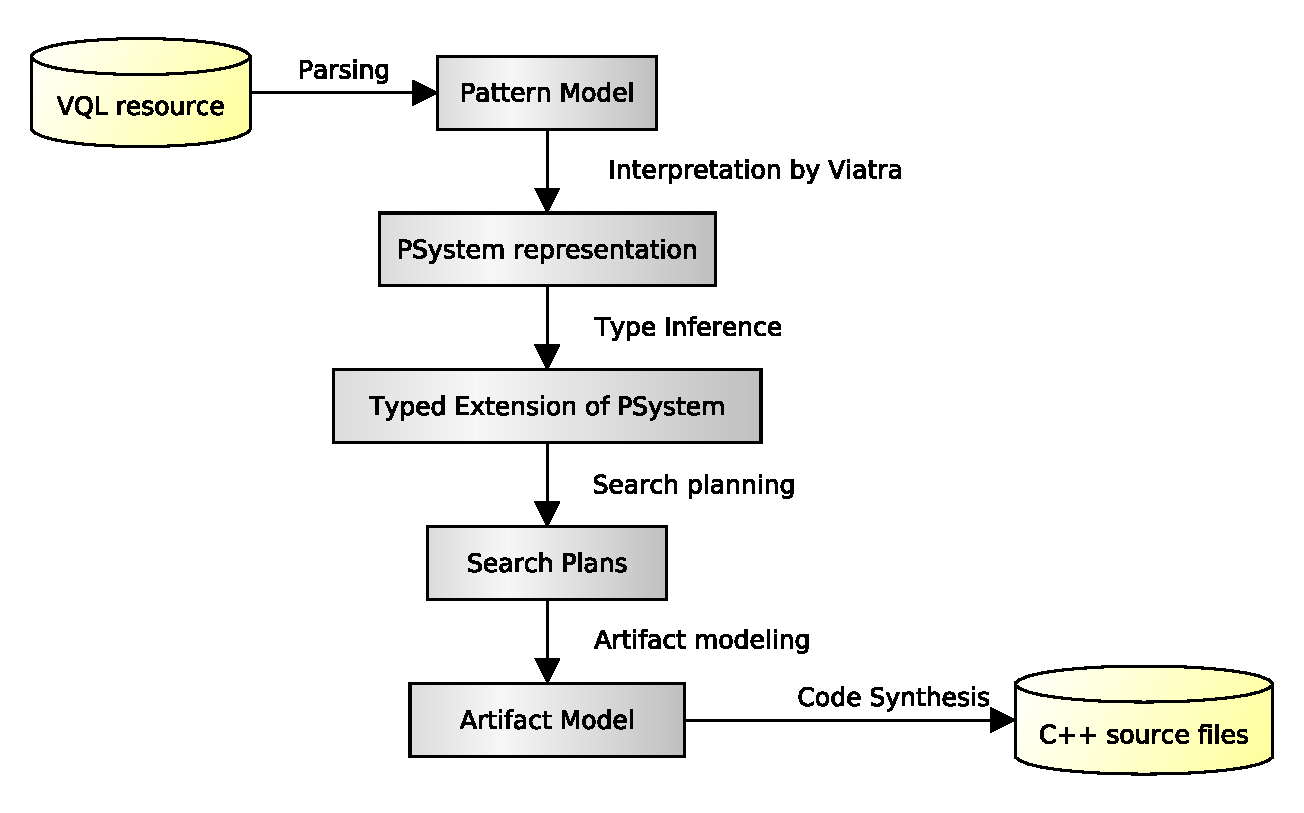
\includegraphics[width=0.8\textwidth]{figures/query-compilation-workflow.pdf}
		\caption{Query compilation workflow}
		\label{figure:query-compile-workflow}
	\end{center}
\end{figure}



\subsection{PSystem representation}


The vql file is loaded into a PatternModel, which is a model for vql files. 
The framework does not use this representation, but passes it to \viatra, which creates its own representations of it called PSystem. \cite{psystem}. 


\begin{figure}
	\begin{center}
		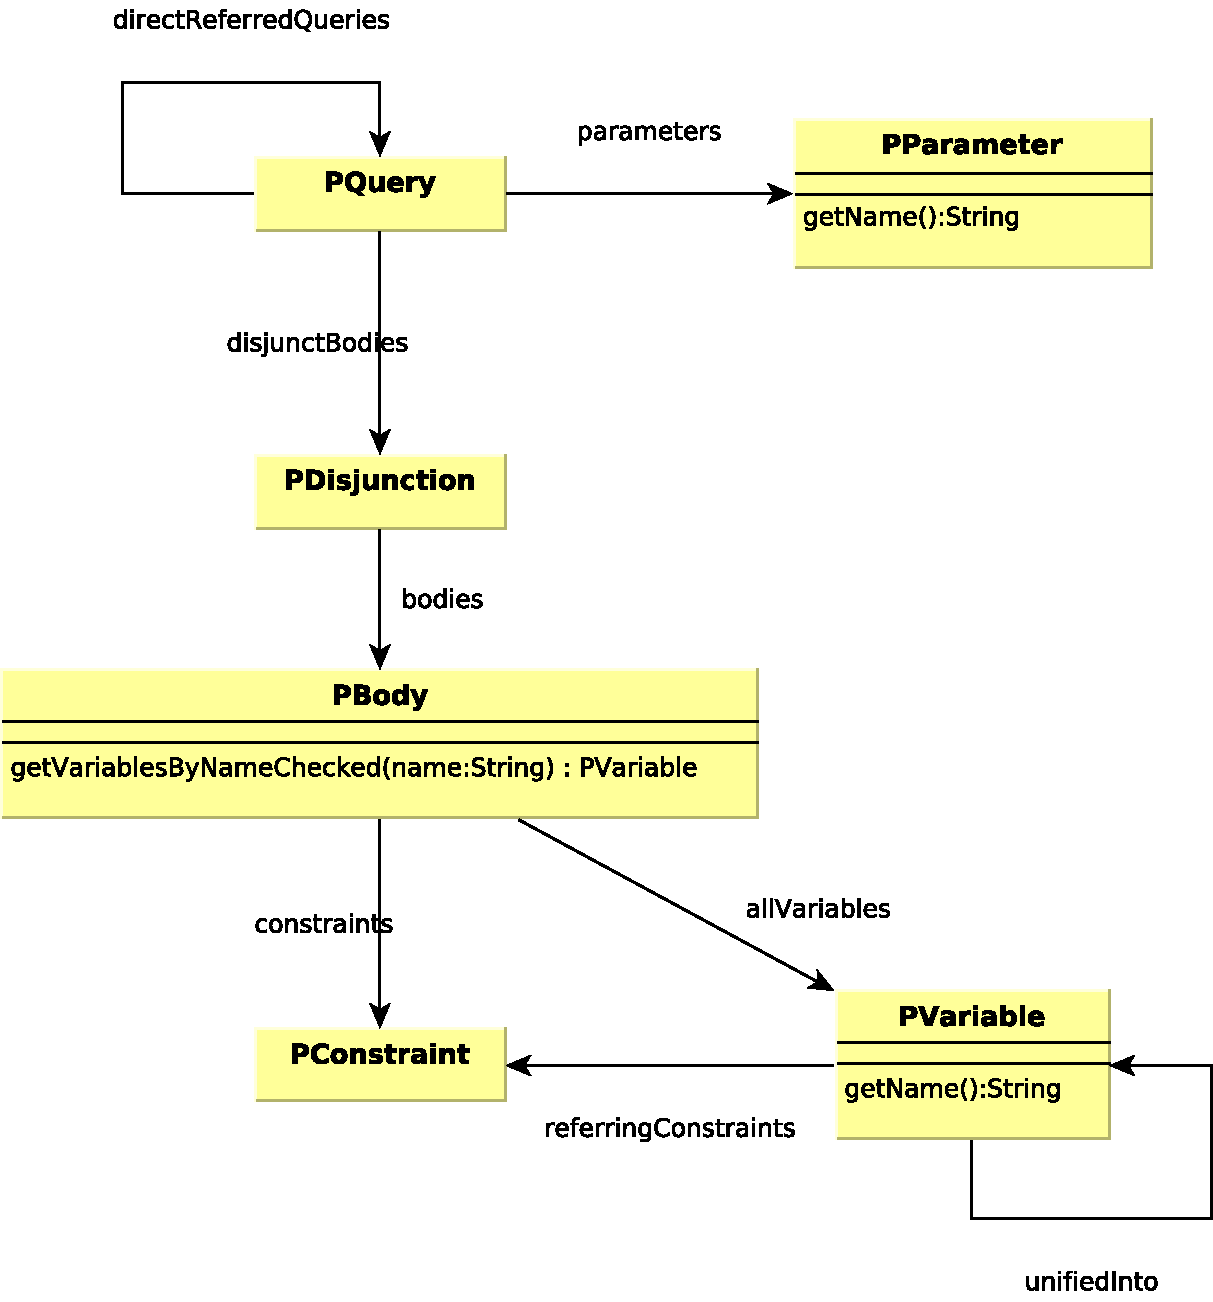
\includegraphics[width=0.6\textwidth]{figures/psystem.pdf}
		\caption{PSystem's structure}
		\label{fig:psystem}
	\end{center}
\end{figure}
The structure of PSystem representation is shown on Figure~\ref{fig:psystem}. 
As their implementation is hidden behind interfaces, most of the refrences means getter functions (In Xtend, gettern functions can be used with field access syntax like \csharp{} properties). 
Graph patterns are represented by a PQuery. 
A PQuery has a parameter list. 
The most important attribute of parameters are its names. 
A PQuery consists of a PDisjunction, which consists of a set of PBodies. 
PDisjunctions play role in Query rewriting, where the bodies of a PQuery gets optimized, or changed other ways.
PBody consists of PConstraints. 
PConstraint is a basic interface for various constraints. 
Altough constraints refer to variables, all variablesin a PBody can be accessed from PBody.

A variable can be unified into another variable. 
This can happen when equality constraint is used between two variable: 
Equality constraint is omitted, one of the variable gets unified into the other, and other constraints do not have to be changed.

%TODO Az ábra még pontosítható
\todo{ Az ábra még pontosítható}


\subsection{Typed Extension of PSystem}

To make PSystem more usable we extend it with additional information, mainly with type information for variables and parameters.
For this the types of the variables and parameters must be infered based on type constraints of the graph pattern.

First the types of the variables must be infered. 
First, we collect all the type constraints, that the variable must satisfy.
We do this, by collecting all the variables that are the same as the variable( via equality constraint eg. ), 
then collect the constraints refering to them.
From this we can create a set of candidate types.
Then we choose the type as the following. 
If the types contains classes and datatypes, then we throw an error.
If all the types are data types, then they must be compatible with each other (integral types, or the same type).
In this case, the most specific is choosen. If there are uncompatible types, then we throw an error.
If all the types are EClass types, then we select the most general class, that are compatible (extends it or is the same) of all the classes and choose that.
If we cannot choose such EClass, or there are multiple classes that satisfies this, then we throw an error (The later can happen eg., when there are two classes, A and B, and exists two class, that are a descendant of both of them).


\begin{figure}[h]
	\begin{center}
		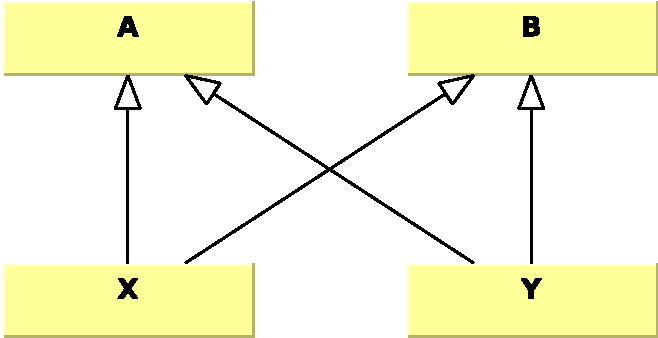
\includegraphics[width=0.4\textwidth]{figures/multiple-inheritance-problem.pdf}
		\caption{Problems with type inference in case of multiple inheritance}
		\label{fig:multiple-inheritance-problem}
	\end{center}
\end{figure}

If the types of the variables are known then the types of the parameters can be infered. 
For this, we collect the variables that represents this parameter from each body.
As the parameters value can be any of the variable, we choose the type, that generalizes them.

We also maintain additional information in our representation. 
Bodies also maintain the relationship between variables and parameters. 
In PSystem, this information is not directly available, parameters and variables need to be matched by name.

\subsection{Search planning}

After we have extended PSystem with the needed information, we can plan how the pattern will be executed.
From a set of constraints that declaratively defines the pattern we need to create an imperative sequence of search operations.

For this, we use the local search planner of \viatra{}.
This planner takes a cost function, then creates a permutation of constraints that minimizes the cost function. 
After this permutation is achieved, then search operations will be created by mapping the constraints to them considering their position.
The cost function must give an approximated cost of applying a constraint based on the variables bound before the application and other information (Like statistics on the instance model, that can only be available at runtime, so \viatra{} can utilize them, but we can't as we generate the monitoring components at design time). 

For the different constraint applications we use the following search operations.

\subsubsection{Type constraint}
If a variable must be of a given type, then the following two search operation can be the next:
If the variable is bound, we need to check wether the already bound value is of that type, we denote this CheckInstanceOf(Var, Type).
If the variable is unbound, we need to iterate over the instances of the type and follow the algorithm, we denote this ExtendInstanceOf(Var, Type) ).


\subsubsection{Reference and attribute constraint}

If a structural feature is \todo{befejezni innentől ezt a fejezetet}


\subsubsection{Negative pattern application}


\subsubsection{Transitive closure}





\subsection{Additional optimization}

After we complete the plan with type information and other details, it can be used to generate C++ code, although before that step we use further optimizations. 
These optimizations considers distributed execution of the plan, so it can improve the plan generated by \viatra{} which is generated to be used in a single computer.


\subsubsection{Replace pattern calls with simpler operations}
There are some cases, where helper patterns are simple, and used to define simple conditions. 
In this case, evaluationg the subquery is not always the most efficient method, sometimes these can be replaced by simple search operations:

\subparagraph{Reference Pattern}
We use the phrase \emph{reference pattern} for a pattern with 2 parameters if its only constraint is that a reference exist between the two parameters, eg.:
\begin{lstlisting}[language = vql]
private pattern connected(a : RailRoadElement, b : RailRoadElement){
	RailRoadElement.connectedTo(a,b);
}
\end{lstlisting}

In the following examples i will use this query as an example to demonstrate how the application of this query can be replaced by an other operation.

\subparagraph{Counting reference pattern} 

\begin{lstlisting}[language = vql]
1 == count find connected(a, _);
\end{lstlisting}


\subparagraph{Negative application of a reference pattern}

\begin{lstlisting}[language = vql]
neg find connected(a, _);
\end{lstlisting}

\subsubsection{Filter unnecessary operations, checks}
As the original plan is generated by the localsearch planner of \viatra{}, there can be redundant operations, which can be ommited. This includes:

\begin{itemize}
	\item Check operation -- The generated code is strongly typed, so we don't need type checks in most cases, unlike in the Java implementation, where the tuples contains plain java objects with unknown types.
	
	\item Distribution operations -- \todo{KIFEJTENI}
\end{itemize}



\subsection{C++ code generation}

The completed and optimized plan are used to generate \cpp{} code. 
Two main methods can be used to run local search plan in case of generated code. 
One is to generate the plan as a data structure and create an interpreter that uses that plan to find matches. 
The other is to generate the code directly from the plan. 
The first method is good if we want to change the plan at runtime, but the interpreter itself introduces an overhead, causing performance to be slower.
We used the later, because we don't change the plan at runtime.













%
\chapter{Runtime execution}
%


\section{Distributed runtime model}

As it has been stated before, the model of the system is stored distributedly on different computation unit. A model element only stored in a given computation unit. References can occur between elements in different partitions, so we create proxy objects, that represents an object from another partition, and the local object stores reference to that object. For example, on figure~\ref{fig:distrib-model-example} this can be seen. There are three computing units called \texttt{BBB1}, \texttt{BBB2} and \texttt{BBB3}. \texttt{s5}, \texttt{tr1}, \texttt{s4} and \texttt{s3} are located on \texttt{BBB2}. 

\begin{figure}[h]
	\begin{center}
		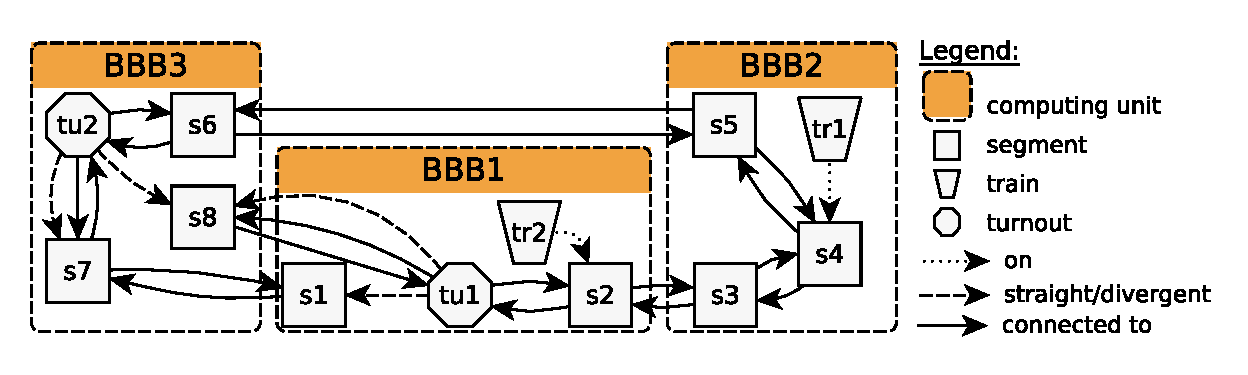
\includegraphics[width=0.9\textwidth]{figures/runtime-snapshot.pdf}
		\caption{Example for a distributed model}
		\label{fig:distrib-model-example}
	\end{center}
\end{figure}




\section{Distributed query execution}


\subsection{Distributed local search}

As models are stored on different computational units we still needs to find matches, that can span over multiple model parts. To find matches for a pattern local search algorithm is used in a distributed way. Search operations are being executed locally, and if the next operation needs to be executed on multiple nodes, the search context, (ie.\ the bound variables and the operations number) are sent to other computational units.

\begin{figure}[h]
	\begin{center}
		\includegraphics[width=1\textwidth]{figures/seq-diagram-query-exec.png}
	\end{center}
\end{figure}
\todo{ábra okosítás}

%----------------------------------------------------------------------------
\chapter{Evaluation}
%----------------------------------------------------------------------------


\section{Measurement setup}

To measure the performance of the code generated by our framework we use the following setup.
We use 6 BeagleBone Black (BBB) \cite{BBB} as computation units. 
We connect them via network. 


\section{Measurement scenarios}

We generated models of size 45, 450, 4500, and 45000.

The models can partitioned to computation units in 3 different ways 
\begin{itemize}
	\item Standard -- The model is partitioned by equally distributing the model considering locality ie.\ elements that are connected have more probability of being allocated to the same unit
	\item Alternative -- The model is partitioned by equally distributing the model not considering locality
	\item Single -- All of the elements are allocated on the same computing unit
\end{itemize}

We measured on this 12 type of models 4 queries: \texttt{closeTrains}, \texttt{derailment}, \texttt{endOfSiding} and\texttt{trainLocations}. 
These were described in Section~\ref{sec:vql-examples}.
We measured the queries time of evaluation 10 times and took their average.

\pagebreak

\section{Results, and evaluation}

The results of the measurements can be seen on \autoref{fig:measurement-interpreted-code}.

\begin{figure}[h]
	\begin{center}
		\includegraphics[width=\textwidth]{figures/measurement-interpreted-code.png}
		\caption{Example for edges between nodes}
		\label{fig:measurement-interpreted-code}
	\end{center}
\end{figure}

The fastest way most of the times were with standard model allocation: it indeed helped to run the queries faster. It was also faster than local evaluation, expect for \texttt{endOfSiding}, where only local model could be measured for the size of 45000, as at other models \texttt{endOfSiding} query was timeouted.

\texttt{trainLocations} and \texttt{closetrains} were faster queries: the reason is obviously the negated pattern call in other queries, which could not be implemented optimally for them.



\chapter{Conclusions}
\label{sec:conclusion}

In this paper we introduced a novel runtime verification system for distributed CPS systems. The approach is based on the VIATRA-Query graph pattern language, which is used to define analysis properties. Graph models are used to define the structural information captured from the system. A code generator generates the data structures and the code to evaluate the queries on the model at runtime. The model is continuously updated with the information received from the environment and fast query execution provides runtime verification. 
The framework combines various technologies from the model-driven and also the CPS domain into a comprehensive approach. A case-study and measurements are used for evaluation purposes. 
The initial measurements show that the approach is capable of analyzing real life systems and the framework can provide fast results even running in microcomputers with low resources.

In the future we plan to continue this line of research. We hope to extend the model handling to provide more adaptability and new strategies have to be added to efficiently handle highly dynamic systems. In addition, we plan to extend the approach to handle temporal properties.
So there is much work left and there are several points where we can further improve the framework. 


% Acknowledgements
%~~~~~~~~~~~~~~~~~~~~~~~~~~~~~~~~~~~~~~~~~~~~~~~~~~~~~~~~~~~~~~~~~~~~~~~~~~~~~~~~~~~~~~
%\include{content/acknowledgement}


% List of Figures, Tables
%~~~~~~~~~~~~~~~~~~~~~~~~~~~~~~~~~~~~~~~~~~~~~~~~~~~~~~~~~~~~~~~~~~~~~~~~~~~~~~~~~~~~~~
%\listoffigures\addcontentsline{toc}{chapter}{\listfigurename}
%\listoftables\addcontentsline{toc}{chapter}{\listtablename}


% Bibliography
%~~~~~~~~~~~~~~~~~~~~~~~~~~~~~~~~~~~~~~~~~~~~~~~~~~~~~~~~~~~~~~~~~~~~~~~~~~~~~~~~~~~~~~
\bibliography{bib/mybib}
\addcontentsline{toc}{chapter}{\bibname}


% Appendix
%~~~~~~~~~~~~~~~~~~~~~~~~~~~~~~~~~~~~~~~~~~~~~~~~~~~~~~~~~~~~~~~~~~~~~~~~~~~~~~~~~~~~~~
%%----------------------------------------------------------------------------
%\appendix
%%----------------------------------------------------------------------------
%\chapter*{\fuggelek}\addcontentsline{toc}{chapter}{\fuggelek}
%\setcounter{chapter}{\appendixnumber}
%%\setcounter{equation}{0} % a fofejezet-szamlalo az angol ABC 6. betuje (F) lesz
%\numberwithin{equation}{section}
%\numberwithin{figure}{section}
%\numberwithin{lstlisting}{section}
%%\numberwithin{tabular}{section}
%
%%----------------------------------------------------------------------------
%\section{Measured queries}
%%----------------------------------------------------------------------------
%
%
%\subsection{Benchmarked patterns}
%
%\begin{lstlisting}[language = vql]
%pattern trainLocations(train: Train, loc: RailRoadElement)
%{
%	Train.on(train, loc);
%}
%\end{lstlisting}
%
%\begin{lstlisting}[language = vql]
%pattern derailment(elem: RailRoadElement, train: Train)
%{
%	Turnout(turnout);
%	RailRoadElement.train(elem,train);
%	
%	neg find connected(elem, turnout);
%	find straightOrDivergent(turnout, elem);
%}
%\end{lstlisting}
%
%\begin{lstlisting}[language = vql]
%pattern CloseTrains(start : RailRoadElement, end : RailRoadElement)
%{
%	
%	Train.on(t1,start);
%	
%	RailRoadElement.connectedTo(start,middle); // Has EOpposite, inverse navigation is effective even without model index
%	RailRoadElement.connectedTo(middle, end);
%	
%	start != end; // This ensures that at least the start and end segment is different
%	
%	RailRoadElement.train(end, t2);
%	
%	t1 != t2; // A train may occupy two neighboring segments when moving; this is not a hazardous situation
%	
%	// Allocation-specific part of the query: global or local execution is based on the substitutions of c1 and c2
%}
%\end{lstlisting}
%
%\begin{lstlisting}[language = vql]
%pattern endOfSiding(train: Train, end: RailRoadElement, neighbor: RailRoadElement)
%{
%	RailRoadElement.connectedTo(end,neighbor);
%	neg find otherNeighbor(end,neighbor,_);
%	
%	RailRoadElement.train(neighbor, train);	
%}
%\end{lstlisting}
%
%\clearpage
%
%\subsection{Helper patterns for benchmark patterns}
%
%
%\begin{lstlisting}[language = vql]
%private pattern connected(a : RailRoadElement, b : RailRoadElement){
%	RailRoadElement.connectedTo(a,b);
%}
%\end{lstlisting}
%
%\begin{lstlisting}[language = vql]
%private pattern straightOrDivergent(turnout : Turnout, elem : RailRoadElement){
%	Turnout.straight(turnout, elem);
%} or {
%	Turnout.divergent(turnout, elem);
%}
%\end{lstlisting}
%
%\begin{lstlisting}[language = vql]
%private pattern otherNeighbor(e : RailRoadElement, n1 : RailRoadElement, n2 : RailRoadElement){	
%	RailRoadElement.connectedTo(e,n1);
%	RailRoadElement.connectedTo(e,n2);
%	n1 != n2;
%}
%
%\end{lstlisting}
%
%\vfill
%
%%----------------------------------------------------------------------------
%%\clearpage\section{Measured queries}
%%----------------------------------------------------------------------------
%


%\label{page:last}
\end{document}
